\RequirePackage{lineno}
\documentclass{revtex4}
%\usepackage[pdftex]{graphicx}

\usepackage{amsmath,amsfonts,amssymb}
\usepackage[english]{babel}
\usepackage[latin1]{inputenc}
\usepackage[T1]{fontenc}
\usepackage{color}
\usepackage{float}
\usepackage{verbatim}
\usepackage{graphicx}
\usepackage{bm}
\usepackage{mathtools}
\usepackage{stmaryrd}
\usepackage{anyfontsize}

\usepackage[font={small}]{caption}
\usepackage{subcaption}
\captionsetup{compatibility=false}
\usepackage{xr}
\externaldocument[extfig-]{msv6}
%\usepackage{epstopdf}
%\usepackage{array}
%\usepackage{tabularx}
%\usepackage{multirow}
\usepackage{color}
%\usepackage{multibox}
%\usepackage{rotating}
% \usepackage{lineno}

%\usepackage[left]{lineno}
%\usepackage[comma,sort&compress]{natbib}
%\usepackage{authblk}
%\usepackage{multicol}

\linespread{1.5}

\usepackage{natbib}
\bibpunct{(}{)}{,}{a}{}{;}

% \bibliographystyle{prsb}

% \usepackage{bibunits}

\newcommand{\beginsupplement}{%
        \clearpage
        \setcounter{table}{0}
        \renewcommand{\thetable}{S\arabic{table}}%
        \setcounter{figure}{0}
        \renewcommand{\thefigure}{S\arabic{figure}}%
     }

% \pagewiselinenumbers
\linenumbers
% \setlength\linenumbersep{3pt}

\begin{document}

% \Blindtext
%\title{Simple rules yield complex communities: deconstructed species interactions and the assembly of communities}
%\title{Community assembly and dynamics by the deconstruction of species interactions}
\title{Supplementary Figures: Eco-evolutionary dynamics and collective dispersal: implications for salmon metapopulation robustness}
\author{
Justin D. Yeakel${}^{1,2,*}$, Jean P. Gibert${}^{1}$, Peter A. H. Westley${}^{3}$, \& Jonathan W. Moore${}^{4}$ \\
${}^1$School of Natural Sciences, University of California, Merced, Merced CA, USA \\
${}^2$The Santa Fe Institute, Santa Fe NM, USA \\
${}^3$College of Fisheries and Ocean Sciences, University of Alaska, Fairbanks, Fairbanks AK, USA \\
${}^4$Earth${}_2$Oceans Research Group, Simon Fraser University, Vancouver BC, Canada \\
${}^*$To whom correspondence should be addressed: jdyeakel@gmail.com
}

\maketitle

\beginsupplement




\begin{figure}
  \captionsetup{justification=raggedright,
singlelinecheck=false
}
\centering
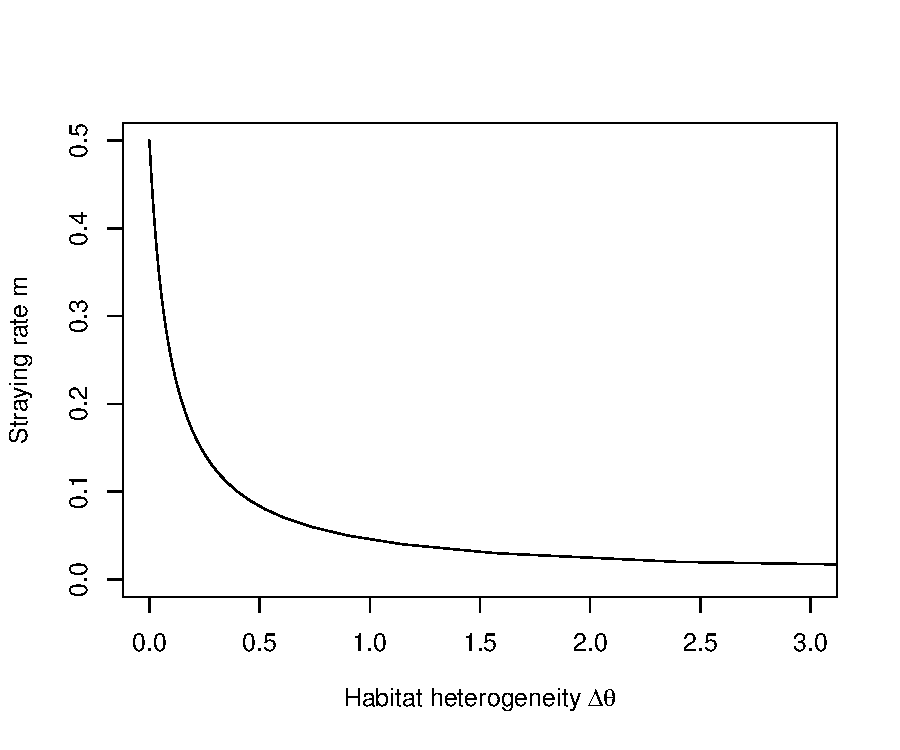
\includegraphics[width=0.35\textwidth]{fig_mthetarelation.pdf}
\caption{
In some cases, habitat heterogeneity may be assumed to determine the rate of straying, if for example:
1) sites are distributed over greater spatial distances, where habitat differences are assumed to be greater between more distant sites, or 2) individuals have behaviors promoting dispersal between habitats that are more similar. To examine such cases, we use the relationship $m= 0.5(1 + \Delta\theta)^{-1}$ where maximum straying is assumed to occur at $m=0.5$ (perfect mixing).
} \label{fig:mthetarelation}
\end{figure}


\begin{figure}
  \captionsetup{justification=raggedright,
singlelinecheck=false
}
\centering
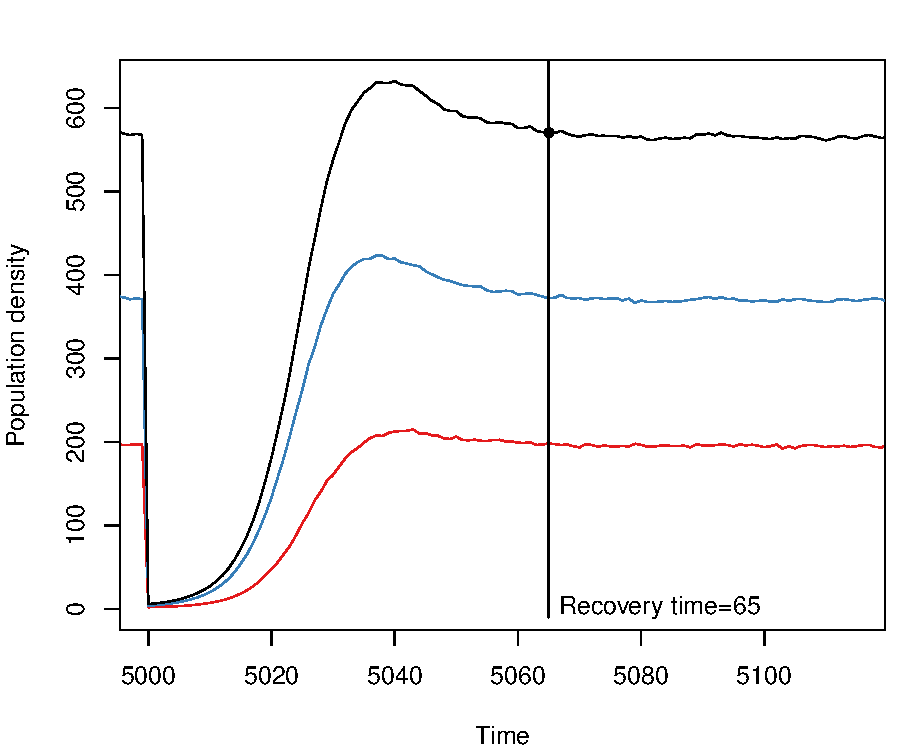
\includegraphics[width=0.35\textwidth]{fig_recovery.pdf}
\caption{
Example of the numerical procedure used to estimate recovery time. After a disturbance is introduced, the recovery time is calculated by measuring the point in time where $N_T$ (in black), which is the aggregate of both populations (blue, red) settles to within one standard deviation of the new equilibrium $N_T^*$. 
} \label{fig:recovery}
\end{figure}


\begin{figure}
  \captionsetup{justification=raggedright,
singlelinecheck=false
}
\centering
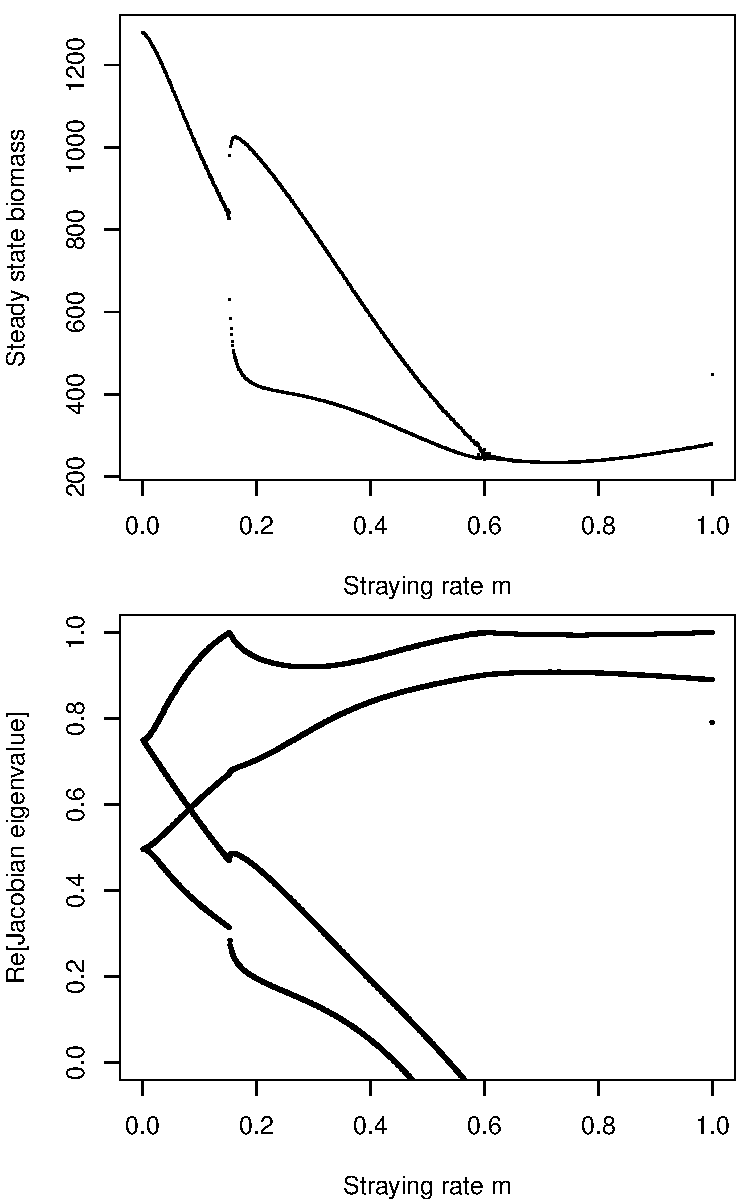
\includegraphics[width=0.35\textwidth]{fig_eigs.pdf}
\caption{
The real parts of the four eigenvalues for the Jacobian matrix of the 4-dimensional system.
The cusp bifurcation occurs when the dominant eigenvalue crosses the unit circle at $+1$. 
} \label{fig:eigs}
\end{figure}


\begin{figure}
  \captionsetup{justification=raggedright,
singlelinecheck=false
}
\centering
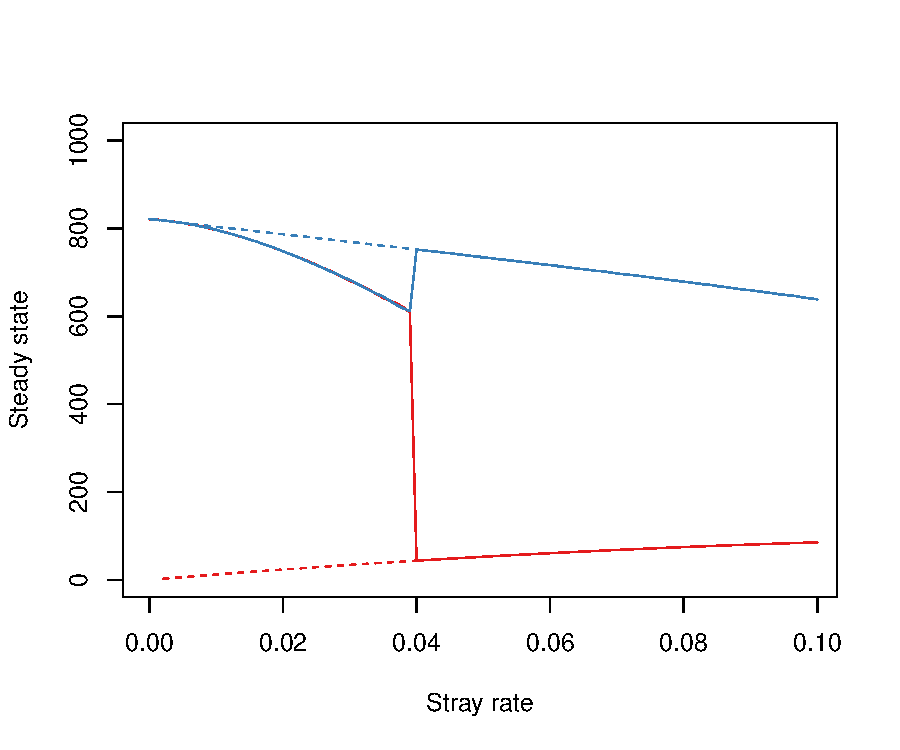
\includegraphics[width=0.35\textwidth]{fig_hysteresis.pdf}
\caption{
Increasing the straying rate results in the transition from a single steady-state for both populations to a dominant and subordinate states. If the straying rate is subsequently lowered, the single steady-state is not easily obtained, which is the hallmark of hysteresis.
} \label{fig:hysteresis}
\end{figure}




\begin{figure}
  \captionsetup{justification=raggedright,
singlelinecheck=false
}
\centering
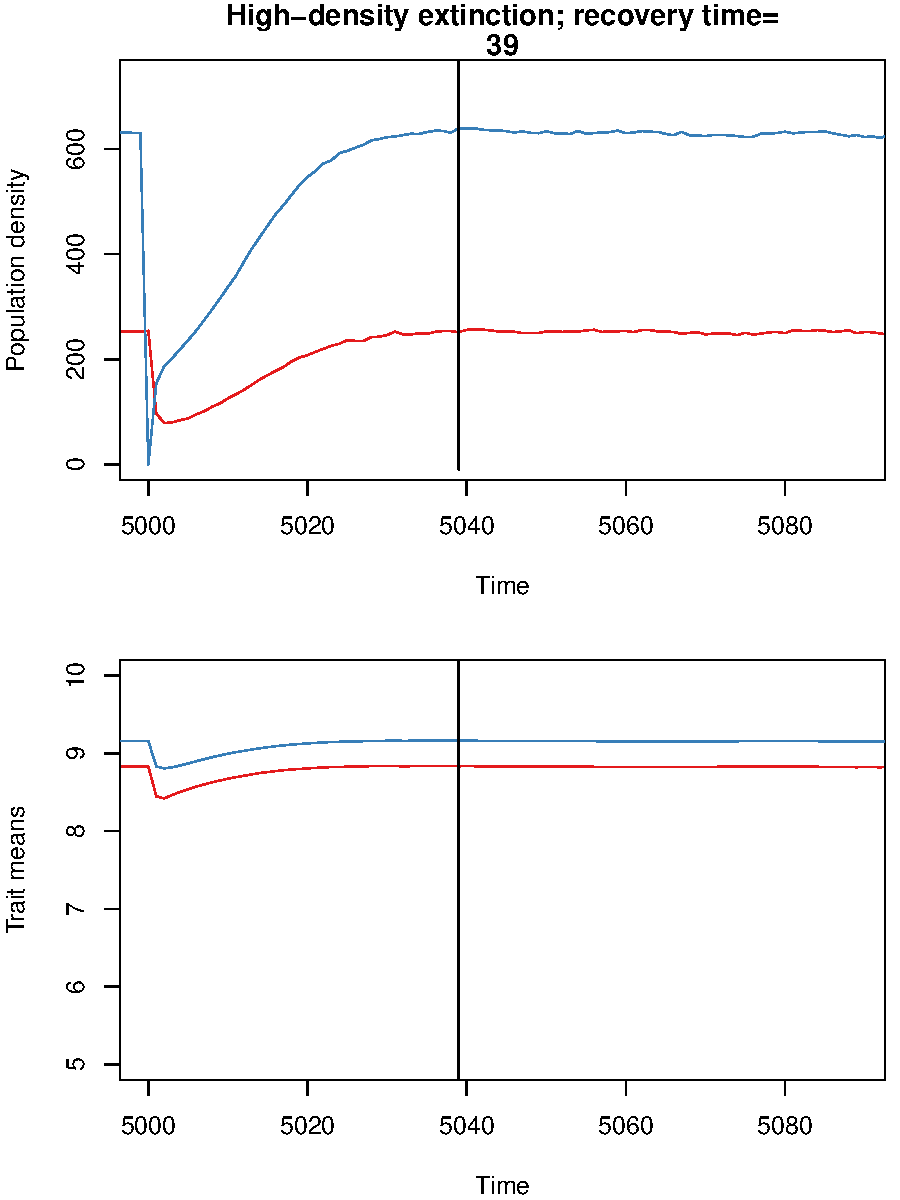
\includegraphics[width=0.35\textwidth]{fig_relax_large.pdf}
\caption{
Extinction of high-density population with a high straying rate $m=0.4$ and low trait heritability $h^2=0.2$ (see figure \ref{extfig-fig:relax}a).
Black line marks the calculated point of recovery post-perturbation.
Trait optima are $\theta_1 = 10$ (blue population trajectory) and $\theta_2 = 5$ (red population).
} \label{fig:relaxtraj_hdlh}
\end{figure}


\begin{figure}
  \captionsetup{justification=raggedright,
singlelinecheck=false
}
\centering
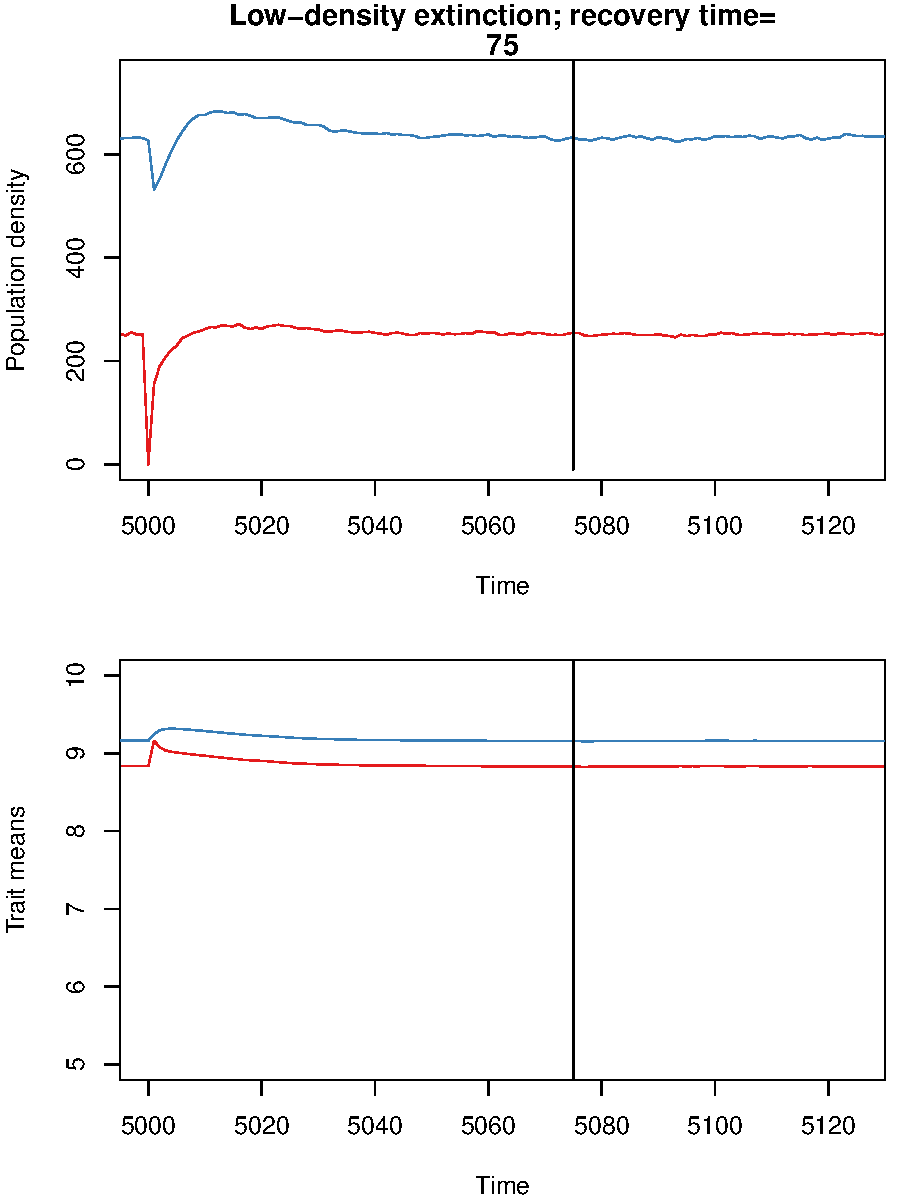
\includegraphics[width=0.35\textwidth]{fig_relax_small.pdf}
\caption{
Extinction of low-density population with a high constant straying rate $m=0.4$ and low trait heritability $h^2=0.2$ (see figure \ref{extfig-fig:relax}a).
Black line marks the calculated point of recovery post-perturbation.
Trait optima are $\theta_1 = 10$ (blue population trajectory) and $\theta_2 = 5$ (red population).
} \label{fig:relaxtraj_ldlh}
\end{figure}



\begin{figure}
  \captionsetup{justification=raggedright,
singlelinecheck=false
}
\centering
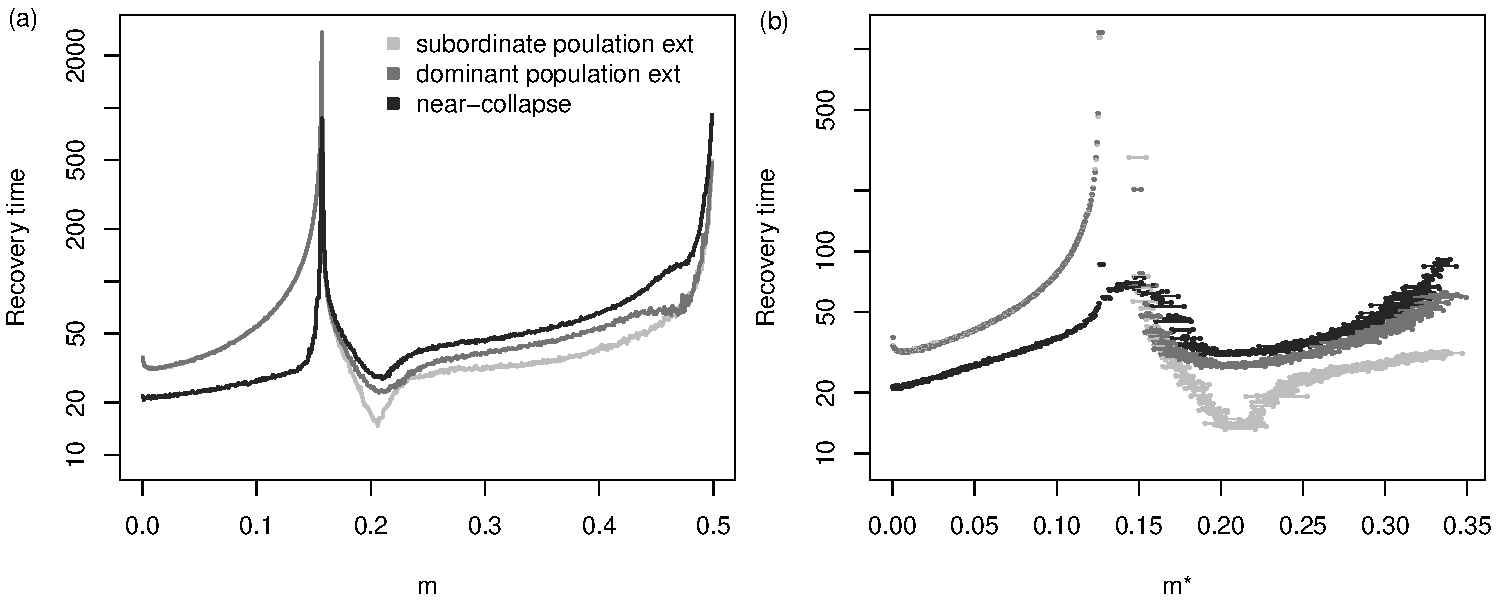
\includegraphics[width=0.9\textwidth]{fig_relax_highh.pdf}
\caption{
Recovery time of $N_T$ following the extinction of either the low-density (light gray) or high-density (gray) population, or the near-collapse of both (dark gray) assuming (a) constant straying rates $m$ and (b) density-dependent straying rates (evaluated at the steady-state $m^*$) with trait heritability $h^2=0.8$.
If $m$ is density-dependent, in the alternative stable state regime there are two straying rates observed: one each for the low- and high-density populations, respectively, which are linked by a horizontal line.
} \label{fig:relax_highh}
\end{figure}



\begin{figure}
  \captionsetup{justification=raggedright,
singlelinecheck=false
}
\centering
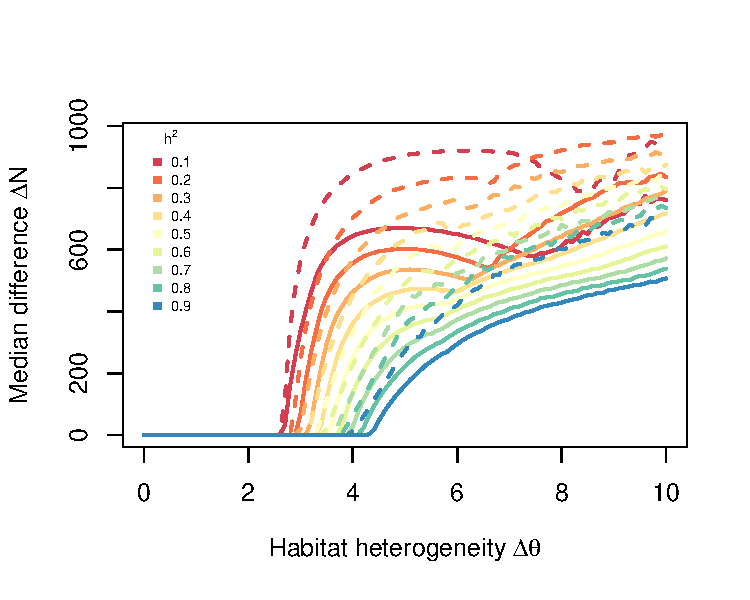
\includegraphics[width=0.4\textwidth]{fig_thetadiffN.pdf}
\caption{
Median difference in population densities taken over the straying rate as a function of habitat heterogeneity $\Delta\theta$.
Solid lines are for constant $m$; dashed lines are for density-dependent $m$.} \label{fig:thetadiffN}
\end{figure}


\begin{figure}
  \captionsetup{justification=raggedright,
singlelinecheck=false
}
\centering
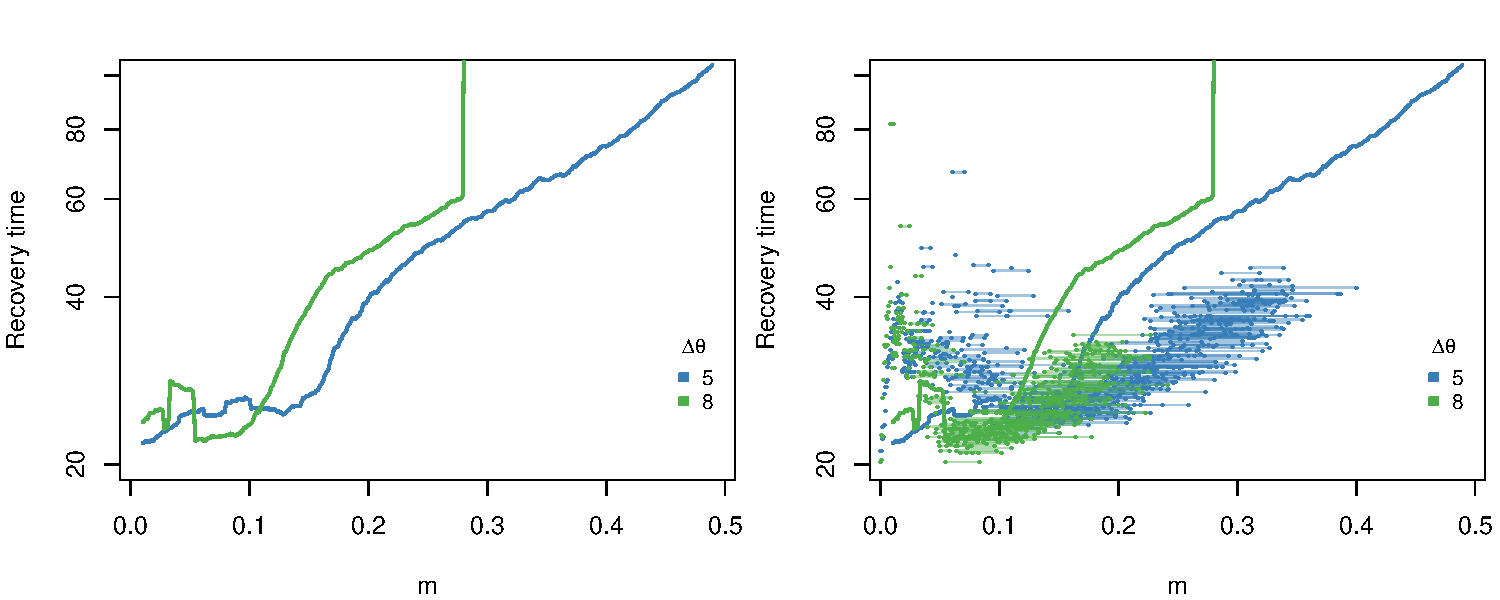
\includegraphics[width=0.8\textwidth]{fig_relaxtheta2.pdf}
\caption{
(a) Recovery time after near collapse of both populations as a function of straying rate $m$ and habitat heterogeneity $\Delta\theta$.
(b) The same as (a) but including recovery times when straying is density-dependent evaluated at $m^*$, shown by linked point pairs.
Recovery times for systems with density-dependent straying are longer when straying is low and shorter when straying is high, mirroring the change in portfolio effects with respect to density-dependent straying shown in figure \ref{extfig-fig:thetaPE}.
} \label{fig:relaxtheta}
\end{figure}



\begin{figure}
  \captionsetup{justification=raggedright,
singlelinecheck=false
}
  \centering
  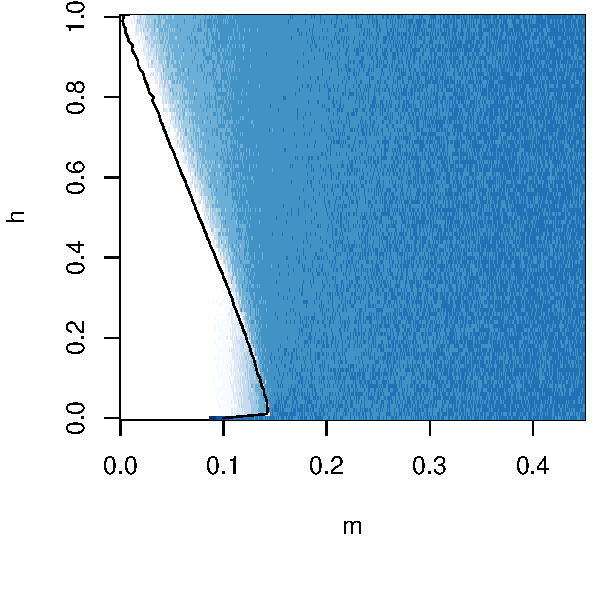
\includegraphics[width=0.35\textwidth]{fig_MDPE_hm_mtheta_rt.pdf}
  \caption{
  Portfolio effects as a function of straying rate $m$ and trait heritability $h^2$ when the rate of straying is $m = 0.5(1 + \Delta\theta)^{-1}$. Alternative steady-states emerge for low values of $m$ (left of the cusp bifurcation, denoted by the black line), whereas a single steady-state exists for high $m$.
  } \label{fig:mthetaPE}
\end{figure}

% \clearpage

\begin{figure}
  \captionsetup{justification=raggedright,
singlelinecheck=false
}
\centering
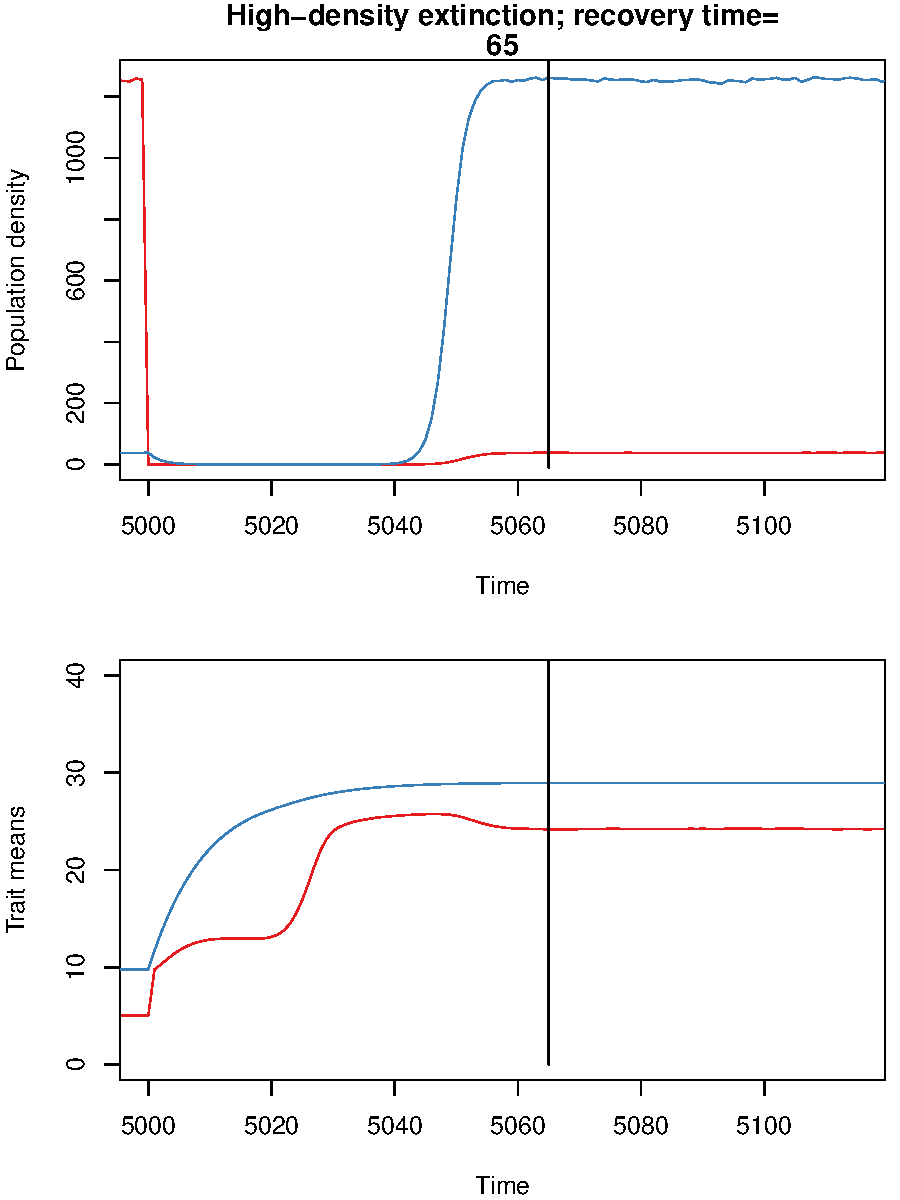
\includegraphics[width=0.35\textwidth]{fig_relax_inertia.pdf}
\caption{
Population inversion where increased differences in trait optima between sites $\Delta\theta$ corresponds to lower rates of straying $m$.
At low rates of straying $m=0.02$ ($\Delta\theta=24$), extinction of the dominant population leads to slower-than-expected recovery times because the subordinate population is isolated enough to evolve towards its own trait optimum. %until growth of the dominant population overwhelms this local selection.
In this case, $m$ is less than $m=0.034$ (denoted by the asterisk in figure \ref{extfig-fig:mtheta}), such that isolation allows the subordinate population to `run away' from the influence of the dominant population.
This leads to a switch in subordinate/dominant states for the two populations.
If $m$ is low but greater than $0.034$, isolation permits the subordinate population to `run away' from the influence of the dominant population, until it is overwhelmed by the recovering dominant population, and reverts back to its previous trait mean prior to disturbance.
} \label{fig:inertia}
\end{figure}


\begin{figure}
  \captionsetup{justification=raggedright,
singlelinecheck=false
}
  \centering
  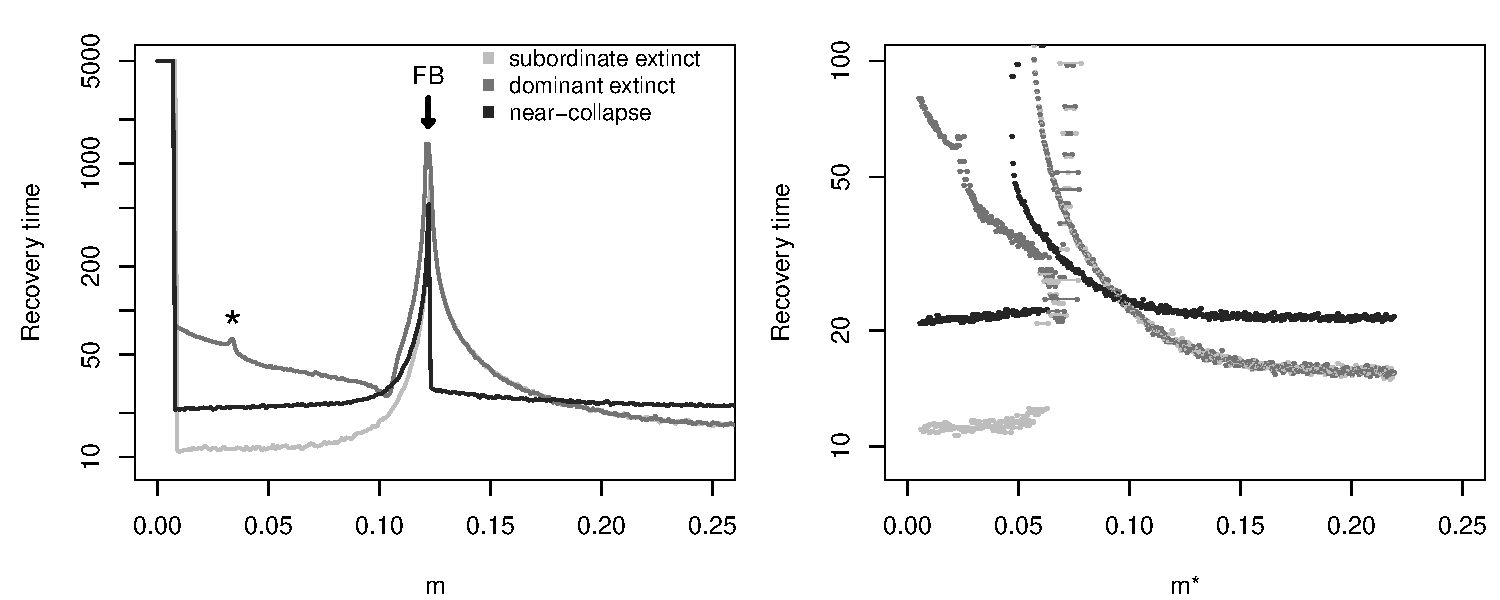
\includegraphics[width=0.8\textwidth]{fig_relax_mtheta.pdf}
  \caption{
  Recovery times for three disturbance types when the straying rate covaries with habitat heterogeneity as $m = 0.5(1 + \Delta\theta)^{-1}$ for constant (a) and density-dependent (b) straying rates.
  The cusp bifurcation is not as clear in (b) because $\Delta\theta$ is a function of the individual straying rate $m_0$, whereas the x-axis in (b) is the straying rate at the steady-state $m^*$.
  Despite this difference, the general behavior shown in (a) are the same in (b).
  } \label{fig:mthetamvm}
\end{figure}

\begin{figure}
  \captionsetup{justification=raggedright,
singlelinecheck=false
}
\centering
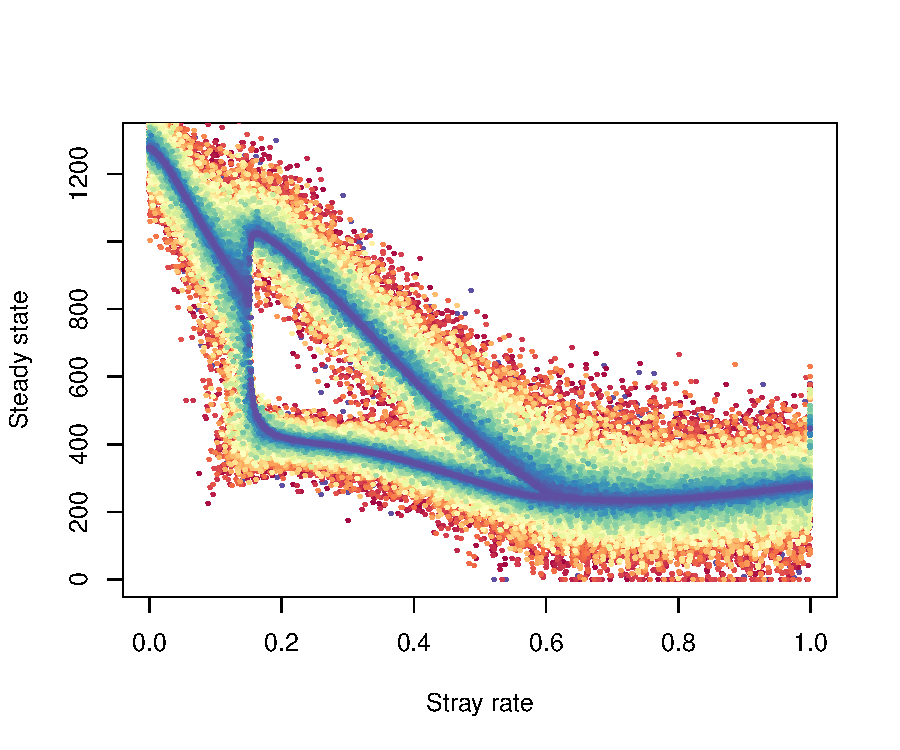
\includegraphics[width=0.35\textwidth]{fig_asymdensity.pdf}
\caption{
Steady-state densities of both populations as a function of $m$, where a cusp bifurcation indicates the emergence of alternative steady-states: one in a dominant state and one in a subordinate state.
Steady-states for populations with symmetrical values ($\alpha=0$) in the vital rates $r_{\rm max}$ and $\beta$ are shown with cool tones.
As the asymmetry among populations between sites increases ($\alpha>0$), their vital rates diverge, such that the maximal growth at sites 1 and 2 is now $r_{\rm max}(1)=r_{\rm max}(1+\tilde{rv}_1)$ and $r_{\rm max}(2)=r_{\rm max}(1+\tilde{rv}_2)$ where $rv_{1,2}$ are independently drawn from $\rm{Normal}(0,\alpha)$ and $r_{\rm max}=2$. 
Similarly the strength of density dependence is calculated at sites 1 and 2 as $\beta(1)=\beta(1+\tilde{rv}_1)$ and $\beta(2)=\beta(1+\tilde{rv}_2)$ where $\tilde{rv}_{1,2}$ are independently drawn from $\rm{Normal}(0,\alpha)$ and $\beta=0.001$.
Steady-states for populations with increasingly asymmetric values ($\alpha\rightarrow 0.1$) for vital rates $r_{\rm max}$ and $\beta$ are shown in warmer tones.
} \label{fig:symmetry}
\end{figure}


\begin{figure}
  \captionsetup{justification=raggedright,
singlelinecheck=false
}
\centering
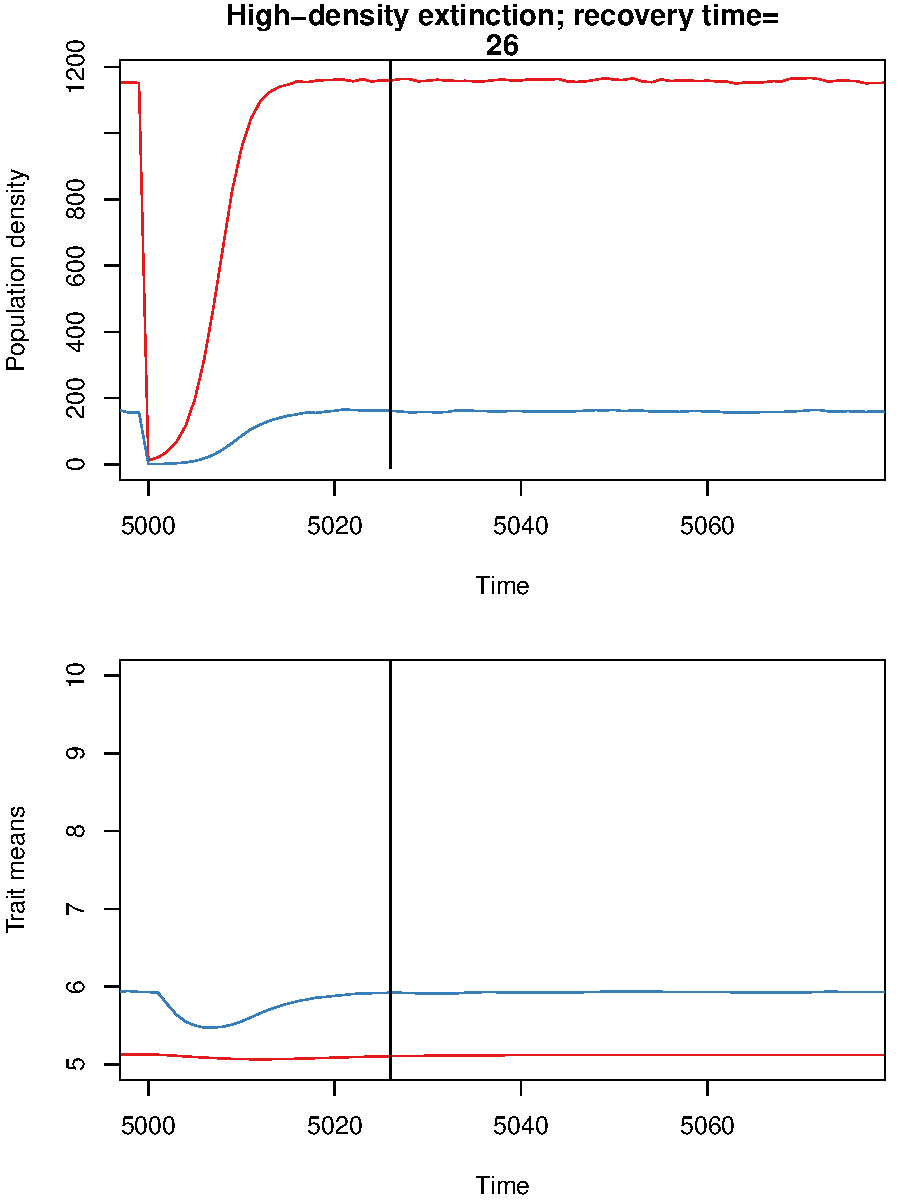
\includegraphics[width=0.35\textwidth]{fig_relax_both_lowh.pdf}
\caption{
Near collapse of both populations with a low straying rate $m=0.1$ and low trait heritability $h^2=0.2$ (see figure \ref{extfig-fig:relax}a).
Black line marks the calculated point of recovery post-perturbation.
Trait optima are $\theta_1 = 10$ (blue population trajectory) and $\theta_2 = 5$ (red population).
} \label{fig:relaxtraj_bothlh}
\end{figure}



\end{document}
